\documentclass[12pt, a4paper, twocolumn]{article}
\usepackage{fontenc, xunicode, xltxtra}
\usepackage{setspace}
\usepackage{geometry}
\usepackage{graphicx}
\usepackage{upgreek}
\usepackage{enumitem}
\usepackage{caption}
\usepackage{titlesec}

\setlength{\parindent}{0pt}
\geometry{a4paper,left=2.5cm,right=2.5cm,top=2.54cm,bottom=2.54cm}
\setmainfont{Times New Roman}
\setlength{\parskip}{6pt}
\renewcommand{\baselinestretch}{1.0}
\captionsetup{font={footnotesize}}  % 调整表格标题字体大小
\titlespacing{\subsection}{0pt}{12pt}{6pt}

\title{COMP90025 Assignment 1B}
\author{Yunlu Wen (yunluw)\ ID: 869338\\ Renjie Zhong (renjie)\ ID: 961201}

\begin{document}
    \maketitle

    \section{Base Algorithm}
    Brute-force solution was chosen as base algorithm for simplicity. What it does is simply trying all the possible combinations of whether using the item or not, so the complexity is $O(2^n)$ where n is the number of items available.

    \section{Parallelization}
    In order to parallelize the algorithm with MPI, we divided the ``used" vector which records the usage of items in to two parts. The most significant K bits are used as counter, which works like a unique id of a job that is distributed to workers. Job ids are scattered from rank0 process to all processes. The rest of the vector is a sub problem for the workers to work out. For example, the following vector has a counter of value 3. When a worker receives a job with counter 3, it first calculating the weight of items already in the knapsack, in this case, is the weight of second item. If the weight is less than the capacity C, then it goes through the brute force algorithm on rest part which maximize the value of items. Otherwise, it simply returns -1 or current value as a result. With this method, the rank0 process only need to broadcast the weight and value vector and job counters to other processes.

    \begin{table}[h]
        \centering
        \begin{tabular}{|c|c|c|c|c|c|c|c|}
            \hline
            0 & 1 & 0 & x & x & x & x & x\\
            \hline
        \end{tabular}
    \end{table}

    The K was chosen to be: 
    $$min(\frac{len(used)}{2}, \log_2(size*2))$$
    where $size$ is number of processes launched in MPI.

    \section{Termination}
    Suppose we have $K$ bits for job counter, then when $2^K$th job is finished, the algorithm should stop. The job distribution is done by scattering, if the first job $ID$ in scatter list is already larger or equal to $2^K$, then the $rank0$ sets all job $ID$s to -2, and all the other processes will quit the loop when they see -2. If only the last few $ID$s are greater than $2^K$, those $ID$s will be set to -1. If receiving processes see -1, it will simply return -1 without any calculation. For example, the situation of $K=3$ is shown in following tables:

    \begin{table}[h]
        \centering
        \caption{Unfinished Jobs}
        \begin{tabular}{|c|c|c|c|}
            \hline
            0 & 1 & 2 & 3\\
            \hline
        \end{tabular}
    \end{table}

    Table 2 shows the situation of ``partially finished". $ID$s with values that greater than threshold will be replaced by -1, which causes returning -1 directly by worker.

    \begin{table}[h]
        \centering
        \caption{Partially Finished}
        \begin{tabular}{|c|c|c|c|}
            \hline
            5 & 6 & 7 & -1\\
            \hline
        \end{tabular}
    \end{table}

    Table 3 displays the situation of ``all finished". In this situation, ``-2"s will be scattered to workers as a signal of breaking the event loop.

    \begin{table}[h]
        \centering
        \caption{All Finished}
        \small
        \begin{tabular}{|c|c|c|c|}
            \hline
            -2 & -2 & -2 & -2\\
            \hline
        \end{tabular}
    \end{table}

    \section{Results and Analysis}

    We tested 1 node, 2 nodes, 4 nodes, and 8 nodes, respectively, and each case was tested with a different number of items. What's more, in order to ensure the accuracy of the data, we tested each case three times and took their average as the final result. The results of the test are displayed in the table below, which use second as the unit.

    \begin{table}[h]
        \centering
        \caption{average processing time (s)}
        \scalebox{0.8}{
            \begin{tabular}{|c|c|c|c|c|c|}
                \hline
                num of items & 1 node & 2 nodes & 4 nodes & 8 nodes \\
                \hline
                20 items & 0.008s & 0.005s & 0.003s & 0.006s \\
                \hline
                25 itmes & 0.324s & 0.134s & 0.126s & 0.041s \\
                \hline
                30 items & 7.6s   & 4.3s   & 2.5s   & 1.2s   \\
                \hline
                35 itmes & 246s   & 143s   & 77s    & 37s    \\
                \hline
            \end{tabular}
        }
    \end{table}

    Since we used brute-force method as our base algorithm, in theory every time 5 items are added, the processing time will be increased by 32 times ($2^5$). Moreover, the number of nodes will be inversely proportional to the processing time. And we can see from the actual test data, the results are basically consistent with our predicted results. Only when the number of items is 20, there is a large deviation from our estimate. We speculate that it is because the amount of data processed is too small, and the advantage of using MPI multi-process parallelism has not been realized. It is more clear to display the data in the form of a line chart.

    \begin{figure}[htb]
        \centering
        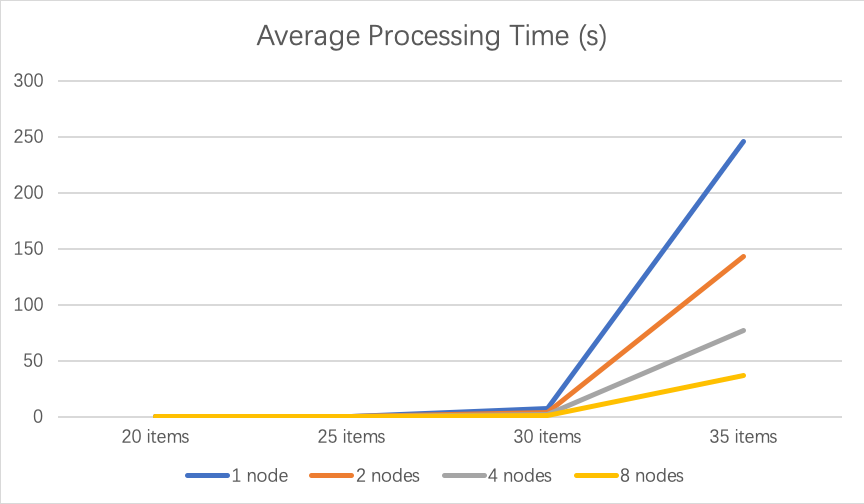
\includegraphics[scale=0.5]{line_chart.png}
        \caption{average processign time (s)}
    \end{figure}

    The relationship between the number of items and the processing time, and the relationship between the number of nodes and the processing time can be clearly seen from Figure 1. In the case of a small number of items, the advantage of using MPI parallelism is not obvious. But as the number of items increases, the advantages of using MPI parallelism are fully reflected. As can be seen from Figure 1, when the number of items is increased to 35, the processing time is significantly inversely related to the number of nodes used.

    \section{Conclusion}
    This report first introduced the algorithm ideas used by our team, and then showed the test data and detailed analysis. After the critical analysis, we came to a conclusion that in the case of small amount of data, MPI has no effect on the processing speed of the algorithm. But when the amount of data increases to a certain extent, the processing speed of the algorithm is proportional to the number of nodes in parallel. The more nodes we use, the faster the processing speed is.

\end{document}